\subsubsection{Дать определение коэффициенту стабилизации параметрического стабилизатор напряжения. Какие существуют пути улучшения этого показателя?}

Параметрические стабилизаторы применяют в случае, когда необходимо получить высокостабильное напряжение и при этом допустимо, что в сопротивлении нагрузки может быть рассеяна малая мощность. В качестве нелинейного элемента, обеспечивающего стабилизацию выходного напряжения, используют стабилитрон. Стабилитроны могут туда ставиться импульсные и двуханодные. Первые для однополярных импульсов, а вторые - для двуполярных. Рассмотрим простейший параметрический стабилизатор:

\begin{center}
	\begin{figure}[h!]
		\center{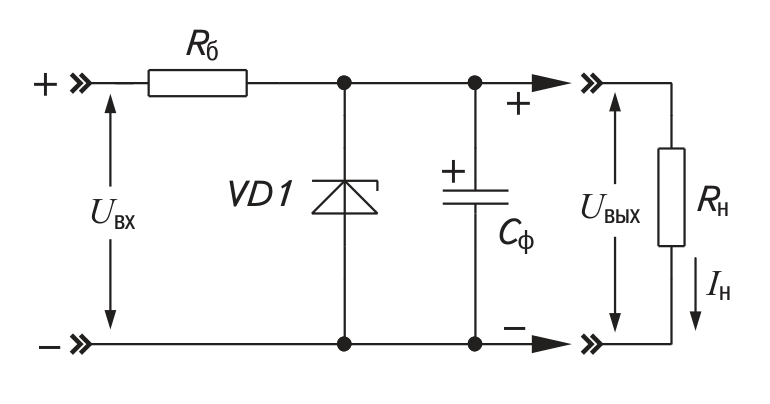
\includegraphics[scale=0.7]{param.png}}
		\caption{Простейший параметрический стабилизатор}
	\end{figure}
\end{center}

и его ВАХ:

\begin{center}
	\begin{figure}[h!]
		\center{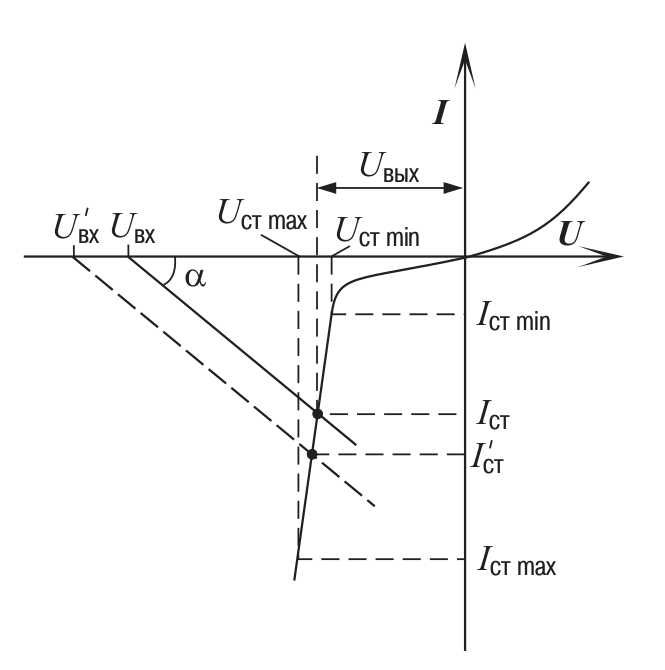
\includegraphics[scale=0.7]{VAHp.png}}
		\caption{Простейший параметрический стабилизатор}
	\end{figure}
\end{center}

Как видно, схема содержит балластный резистор $R_b$ и стабилитрон VD1, который включается параллельно нагрузке. Необходимо обеспечить РТ стабилитрона в пределах, показанных на его ВАХ. Из этих соображений параллельно еще часто включают фильтрующий конденсатор $C_f$. Принцип работы параметрического стабилизатора хорошо виден при рассмотрении нагрузочных характеристик, представленных на ВАХ. Здесь угол наклона прямой определяется сопротивлением балластного резистора $R_b$ (из предположений, что $R_b << r_{st} $). Видно, что выходное напряжение стабилизатора, а также ток стабилитрона определяются положением точки пересечения нагрузочной прямой резистора и ВАХ стабилитрона. Если значение входного напряжения изменится, то изменится и положение рабочей точки, но при этом напряжение на стабилитроне, а значит и на нагрузке останется практически неизменным. 

Итак, пусть изменится входное напряжение. Тогда изменится ток через стабилитрон. Это приведёт к изменению падения напряжения на балластном сопротивлении $R_b$ и к изменению падения напряжения на сопротивлении нагрузки.
$$
\Delta U_{out} = \Delta I_{st}r_{st}
$$
$r_st = \partial U_{st}/\partial I_{st}$ - дифференциальное сопротивление стабилитрона.

Очевидно, что для нашего случая справедливо уравнение
$$
\Delta U_{out} = \Delta U_{in} - \Delta I_{st}R_b
$$

Подставив предыдущее в это получим:
$$
\Delta U_{out}\left(1 + \frac{R_b}{r_{st}} \right) = \Delta U_{in}
$$

Коэффициент стабилизации напряжения будет равен
$$
K_s = \frac{\Delta U_{in}}{U_{in}}\frac{U_{out}}{\Delta U_{out}} = \frac{U_{out}}{U_{in}}\left( 1 + \frac{R_b}{r_{st}}\right)
$$

Отсюда видно, что коэффициент стабилизации напряжения тем больше, чем меньше дифференциальное сопротивление и больше балластное. Но при увеличении $R_b$ меньше будет доставаться нагрузке, так же, как и в случае уменьшения $r_{st}$. В свою очередь, при увеличении нагрузки, всё больший ток будет течь через стабилитрон, будет уменьшаться дифференциальное сопротивление $r_{st}$. Как следствие, ухудшается КПД цепи. Стабилитрон должен предусматривать максимально возможный ток $I_{max} = U_{in}/(R_b + r_{st})$.

\textbf{Пути улучшения коэффициента стабилизации}

Как неоднократно упоминалось в предыдущих вопросах, коэффициент стабилизации есть отношение коэффициента пульсаций на входе к коэффициенту пульсаций на выходе. 

Один из способов улучшить коэффициент стабилизации:
\begin{center}
	\begin{figure}[h!]
		\center{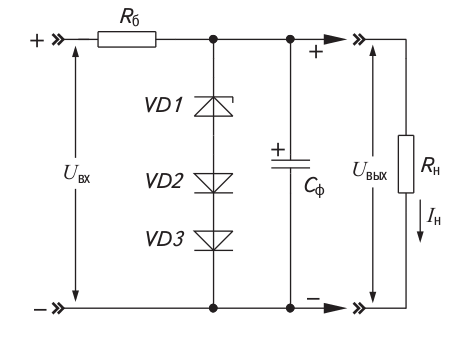
\includegraphics[scale=0.7]{1stw.png}}
		\caption{Простейший параметрический стабилизатор}
	\end{figure}
\end{center}

Как известно, напряжение стабилизации стабилитрона с изменением температуры может смещаться, такое смещение характеризуется параметром, называемым температурным коэффициентом напряжения стабилизации. Для стабилитронов с низким напряжением стабилизации (< 5...6 В) температурный коэффициент напряжения стабилизации имеет отрицательный знак, а для стабилитронов с большим значением напряжения стабилизации — положительный. Для компенсации температурного ухода напряжения стабилизации в параметрические стабилизаторы могут вводиться различные дополнительные элементы. Например, в схеме на рис. выше последовательно со стабилитроном включены два диода в прямом смещении. Такая схема предполагает, что напряжение стабилизации стабилитрона превышает 6 В, а температурный коэффициент напряжения стабилизации составляет около 4 $mV/^{\circ}C$. Известно, что кремниевые диоды в прямом включении имеют отрицательный коэффициент напряжения (порядка –2 $mV/^{\circ}C$), поэтому последовательное включение двух диодов компенсирует температурный уход напряжения стабилитрона.

Следует учитывать, что в таких схемах значение стабилизированного выходного напряжения несколько выше, чем в типовой схеме без диодов, поскольку к напряжению стабилизации стабилитрона в этом случае добавляется падение напряжения на прямосмещенных диодах. При этом существенно увеличивается сопротивление нелинейного элемента, следовательно уменьшается общий коэффициент стабилизации.

Часто применяются мостовые параметрические стабилизаторы:
\begin{center}
	\begin{figure}[h!]
		\center{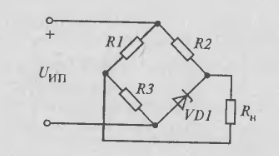
\includegraphics[scale=0.7]{2ndw.png}}
		\caption{Простейший параметрический стабилизатор}
	\end{figure}
\end{center}

В этой схеме повышение коэффициента стабилизации происходит за счёт того, что при изменении $U_{in}$ изменяется и падение напряжения $U_{R_3}$.
При увеличении напряжения входного, увеличивается ток через стабилитрон, а значит увеличивается и напряжение, падающее на нём. Если резисторы $R_1$ и $R_3$ будут подобраны таким образом, что на резисторе $R_3$ в следствие придешдей $\Delta U$ на вход упадёт такая же $\Delta$, как и на диоде VD1, то выходное напряжение практически не изменится.

К минусам данной схемы можно отнести то, что на диоде падает не $U_{st}$

